\hypertarget{duxe9roulement-du-stage-et-travail-ruxe9alisuxe9}{%
\chapter{Déroulement du stage et travail
réalisé}\label{duxe9roulement-du-stage-et-travail-ruxe9alisuxe9}}

Durant les 4 semaines de stage, j'ai été confronté à beaucoup de
nouvelles choses :

\begin{itemize}
\tightlist
\item
  Principes théoriques (Apprentissage / NN / SNN )
\item
  N2S3 \& Scala
\item
  Rédaction \& communication
\item
  Découverte de divers Outils (ssh / ftp / git / cluster de calcul /
  pandoc )
\end{itemize}

Dans cette section, nous aborderons chacun de ces points.

\hypertarget{les-ruxe9seaux-de-neurones-principes}{%
\section{Les réseaux de neurones :
principes}\label{les-ruxe9seaux-de-neurones-principes}}

Pour commencer, je décrirais brièvement le fonctionnement des réseaux de
neurones artificiels impulsionnels. Tout l'intérêt des réseaux de
neurones impulsionnels ne peut apparaitre que si l'on comprend, même
sommairement, ce qui les distingue des réseaux de neurones classiques.
L'ensemble des informations présentées dans cette section sont tirées de
nombreuses discussions avec les membres du groupe \textbf{Spikes} ainsi
que d'un livre (\cite{naturalHandbook})

Voyons donc comment fonctionne un neurone classique avant d'établir des
connections entre eux.

\hypertarget{les-ruxe9seaux-de-neurones-classiques}{%
\subsection{Les Réseaux de neurones
classiques}\label{les-ruxe9seaux-de-neurones-classiques}}

\hypertarget{le-neurone-artificiel-classique}{%
\subsubsection{Le neurone artificiel
classique}\label{le-neurone-artificiel-classique}}

Un neurone biologique, ou une cellule nerveuse, est une cellule
excitable constituant l'unité fonctionnelle de base du système nerveux.
Les neurones assurent la transmission d'un signal bioélectrique appelé
influx nerveux.

Le neurone artificiel classique manipule des valeurs réelles. Il dispose
de plusieurs entrées (\(x_i\)) et d'une sortie. Chaque entrée est
associée à un poids (\(w_i\)) correspondant à l'importance de cette
entrée; ainsi qu'un poids b pouvant être ajouter en complément. Le
neurone calcule la somme pondérée de ses entrées. Cette somme passe
ensuite dans une \textbf{fonction d'activation} \(f\) qui détermine la
valeur en sortie \(o\) du neurone.

Il existe dans la littérature de nombreuses variantes portant notamment
sur la fonction d'activation, mais le principe reste celui ci.

On peut résumer ce fonctionnement par l'équation \ref{eq:neurone} et la
figure \ref{fig:neurone}. \begin{equation}
\label{eq:neurone}
o = f(\sum_i {w_i . x_i })
\end{equation}

\begin{figure}[h!]
\label{fig:neurone}
\centering
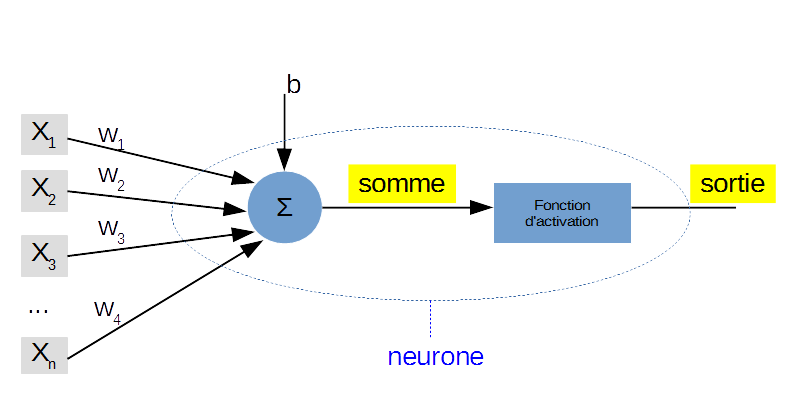
\includegraphics[width=10cm]{./images/neurone.png}
\caption{le neurone classique : principe de base}
\end{figure}

Un neurone est donc une petite unité de calcul dont les résultats
dépendent de ses poids. C'est utilisé en réseau qu'il révèle tout son
intérêt pour l'\textbf{apprentissage supervisé}. Si cette notion n'est
pas familière au lecteur, elle est décrite de façon succincte dans
l'annexe \ref{apprentissage-supervisuxe9}

\hypertarget{ruxe9seaux-de-neurones-pour-lapprentissage.}{%
\subsubsection{Réseaux de neurones pour
l'apprentissage.}\label{ruxe9seaux-de-neurones-pour-lapprentissage.}}

Un réseau est un ensemble d'éléments interconnectés entre eux pour
échanger des informations. Un réseau de neurones artificiels s'inspire
du fonctionnement biologique du cerveau humain et prend corps dans un
ordinateur. Il suffit donc d'associer plusieurs neurones pour établir un
réseau. Il existe plusieurs types de réseaux suivant la façon dont sont
connectés les neurones entre eux.

En apprentissage automatique, le réseau de neurones doit choisir à
quelle catégorie ou \textbf{classe} appartient un objet défini par ses
\textbf{caractéristiques} (\(x\)). Les réseaux de neurones ont alors
souvent la structure décrite ci dessous.

\hypertarget{la-couche-dentruxe9e}{%
\paragraph{La couche d'entrée}\label{la-couche-dentruxe9e}}

Le vecteur \(x\) contenant les caractéristiques de l'objet est introduit
sur la \textbf{couche d'entrée} du réseau. Celle ci présente autant
d'emplacements que le nombre de dimensions du vecteur \(x\).

Exemples : Nous illustrerons nos propos sur des bases bien connues en
apprentissage automatique : la base \textbf{IRIS} et la base
\textbf{MNIST}. Celles ci sont décrites de façon plus précise dans la
section \ref{les-bases-dexemples}.

\begin{itemize}
\tightlist
\item
  si l'on classifie des plantes sur la base de 4 mesures faites sur ces
  plantes (base \emph{IRIS}), la couche d'entrée sera constituée de 4
  neurones.
\item
  si l'on classifie des images de 28x28 pixels (base \emph{MNIST}), la
  couche d'entrée sera constituée de 28x28 = 786 neurones
\end{itemize}

\hypertarget{la-couche-de-sortie}{%
\paragraph{La couche de sortie}\label{la-couche-de-sortie}}

De l'autre côté du réseau se trouve la couche de sortie. Elle est
souvent constituée de la façon suivante : chaque neurone de sortie est
sensé reconnaitre une \textbf{classe} du problème. On peut alors voir
chaque neurone de sortie comme le producteur d'un \textbf{score}
correspondant à l'adéquation entre les entrées \(x\) et la
\textbf{classe} à laquelle le neurone est dédié. La décision finale
prise par le réseau de neurone consiste souvent à observer quel neurone
de sortie a donné le \textbf{score} le plus grand.

Exemples :

\begin{itemize}
\tightlist
\item
  si l'on classifie 3 sortes de plantes (base \emph{IRIS}), la couche de
  sortie sera constituée de 3 neurones.
\item
  si l'on classifie des chiffres (base \emph{MNIST}), la couche de
  sortie sera constituée de 10 neurones.
\end{itemize}

\hypertarget{principe-dapprentissage-des-poids}{%
\paragraph{Principe d''apprentissage des
poids}\label{principe-dapprentissage-des-poids}}

Dans la version la plus simple du réseau de neurones, la couche d'entrée
est directement connectée à la couche de sortie (chaque neurone d'entrée
est connecté à chaque neurone de sortie). C'est le principe d'un
\textbf{réseau de neurone monocouche} tel que celui de la figure
\ref{fig:monocouche}

\begin{figure}[h!]
\label{fig:monocouche}
\centering
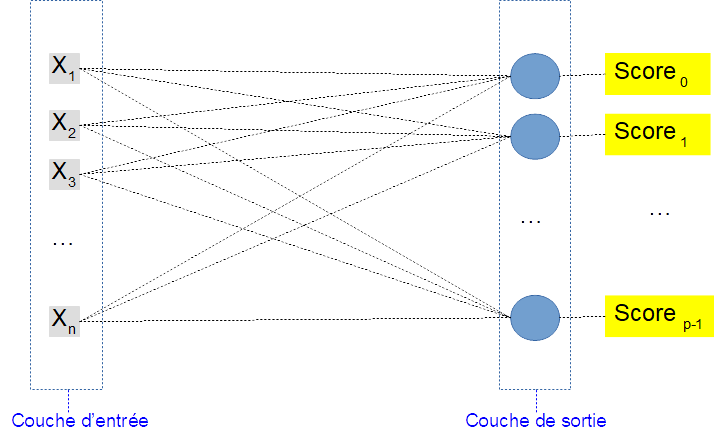
\includegraphics[width=10cm]{./images/monocouche.png}
\caption{réseau monocouche classique}
\end{figure}

Lors d'un apprentissage supervisé :

\begin{enumerate}
\def\labelenumi{\arabic{enumi}.}
\tightlist
\item
  Le réseau est initialisé avec des poids aléatoires (ses décisions sont
  donc complètement arbitraires).
\item
  On présente un exemple (\(x\)) dont la véritable classe est connue
  (\(l\)) sur la couche d'entrées
\item
  On calcule la valeur en sortie de chaque neurone de la couche de
  sortie
\item
  On en déduit la décision du réseau. \((l_nn)\)
\item
  si \(l_nn = l\), le réseau a raison, on ne fait rien. Si
  \(l_nn \neq l\), les poids des connections sont corrigés pour que lors
  de la prochaine présentation de cet exemple, le réseau donne une
  réponse plus proche de la réponse attendue.
\item
  On recommence au point 2. avec un nouvel exemple.
\end{enumerate}

Ce fonctionnement de base est conditionné par la capacité des programmes
à corriger les poids lors de l'étape 5.

Si l'on peut imaginer de nombreuses méthodes de corrections des poids,
on peut également imaginer des architectures plus complexes, visant à
laisser le réseau combiner de façon plus poussées les informations
issues de la couche d'entrée.

\hypertarget{architectures-internes-des-ruxe9seaux-de-neurones.}{%
\paragraph{Architectures internes des réseaux de
neurones.}\label{architectures-internes-des-ruxe9seaux-de-neurones.}}

Il existe de nombreuses variantes d'architectures pour les réseaux de
neurones classiques mais la plus usitée est une architecture de couches
cachées connectées de proche en
proche\footnote{Il faut noter qu'à ce jour, personne ne sait théoriquement comment choisir le nombre de couches cachées ni la taille de ces couches pour un problème donné. Seul la pratique permet d'obtenir des résultats corrects.},
comme celle présentée en figure \ref{fig:multicouche} .

\begin{figure}[h!]
\label{fig:multicouche}
\centering
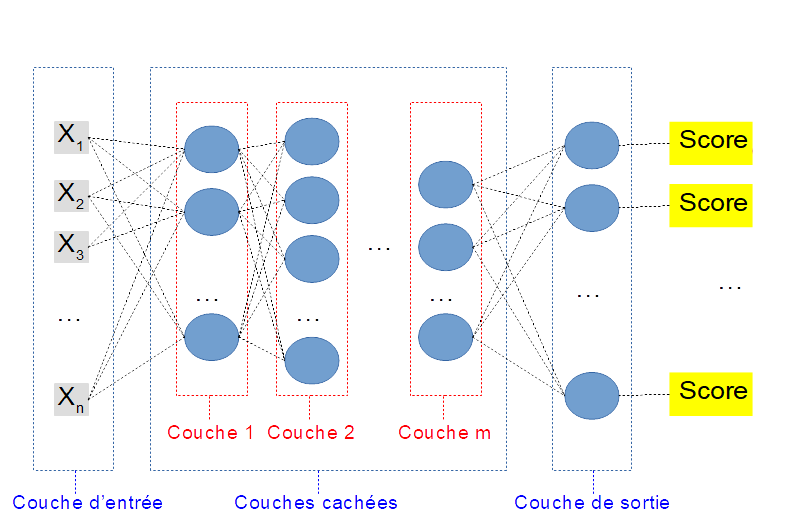
\includegraphics[width=10cm]{./images/multicouche.png}
\caption{réseau multicouche classique}
\end{figure}

Lors d'un apprentissage supervisé : l'algorithme reste semblable à celui
précédemment présenté. Néanmoins, lors de l'étape 5 de l'algorithme
précédent, la correction des poids doit être faite à travers toutes les
couches depuis la couche de sortie, jusqu'à la couche d'entrée. Une
partie des progrès réalisée par les réseaux de neurones s'explique par
la mise au point de techniques fiables dans ce domaine (\emph{la
rétropropagation du gradient} est une de ces techniques)

Une grande partie de ces principes reste valable dans le cas de réseaux
de neurones impulsionnels, c'est pourquoi nous les avons présentées.
Voyons donc plus précisément le cas de ces réseaux qui ont fait l'objet
de ce stage :

\hypertarget{les-ruxe9seaux-de-neurones-impulsionnels}{%
\subsection{Les réseaux de neurones
impulsionnels}\label{les-ruxe9seaux-de-neurones-impulsionnels}}

Encore une fois, commençons par décrire un neurone impulsionnel :

\hypertarget{le-neurone-artificiel-impulsionnel}{%
\subsubsection{Le neurone artificiel
impulsionnel}\label{le-neurone-artificiel-impulsionnel}}

A la différences des neurones artificiels classique, le neurone
artificiel impulsionnel, lui, ne manipule plus des valeurs réelles, mais
manipule des \textbf{spikes} (impulsions) envoyées à une date précise.

Comme le neurone classique, le neurone impulsionnel effectue une somme
de ses entrées. Les entrées étant des impulsions, le mécanisme de
sommation est un peu plus complexe.

\begin{itemize}
\tightlist
\item
  Le neurone est caractérisé par son \textbf{potentiel de membrane} que
  l'on pourrait voir comme le niveau d'excitation du neurone.
\item
  Chaque spike entrant va augmenter ce potentiel de membrane
  proportionnellement au poids de la connection sur laquelle ce spike
  arrive.
\item
  En l'absence de spike entrant, le potentiel de membrane revient vers
  son niveau de repos.
\item
  Si le potentiel de membrane dépasse un seuil à l'instant \(t\), le
  neurone émet un spike à cet instant.
\end{itemize}

Nous pouvons observer ce fonctionnement dans la figure
\ref{fig:neuronSpike}

\begin{figure}[!h]
\label{fig:neuronSpike}
\centering
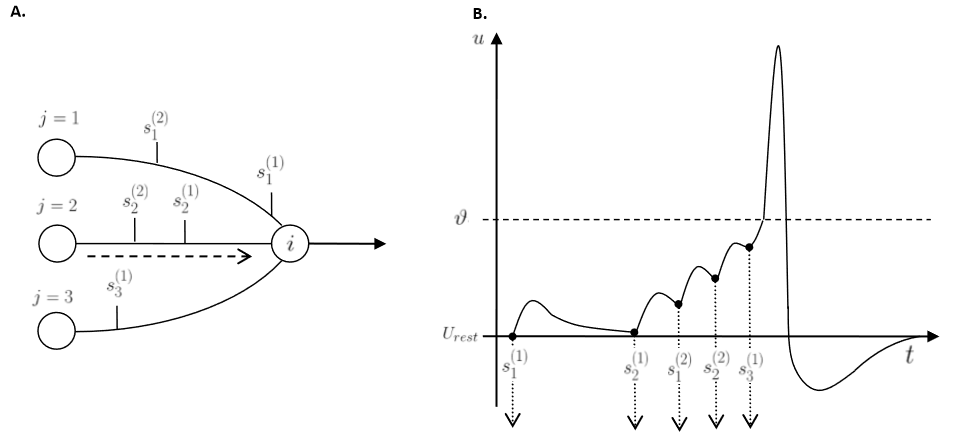
\includegraphics[width=10cm]{./images/image9.png}
\caption{Le neurone impulsionnel : principe de base. \textbf{A} : un neurone et ses entrées. \textbf{B} : le potentiel de la membrane (u) du neurone $i$ en fonction du temps (t). Au fur et à mesure que les spikes du diagramme \textbf{A}. atteignent $i$, on constate une augmentation du potentiel de la membrane, suivie de périodes de baisse. Au fur et à mesure que la densité des spikes augmente à partir de s2 (1), le potentiel atteint le seuil ($\vartheta$), provoquant un spike. Après le spike, le potentiel diminue rapidement vers le potentiel de repos}
\end{figure}

Bien entendu, il existe différentes variantes simulant ce principe de
fonctionnement. L'évolution du potentiel de membrane est en général
gouvernée par une équation différentielle plus ou moins complexe en
fonction du modèle de neurone utilisé.

Ici encore, le neurone impulsionnel est une petite unité de calcul dont
les résultats dépendent de ses poids mais ces neurones n'observent que
la synchronisation existant entre ses entrées.

\hypertarget{ruxe9seaux-de-neurones-impulsionnels-pour-lapprentissage.}{%
\subsubsection{Réseaux de neurones impulsionnels pour
l'apprentissage.}\label{ruxe9seaux-de-neurones-impulsionnels-pour-lapprentissage.}}

Dans les faits, le principe reste le même que détaillé plus haut. Il
faut simplement ajouter quelques précisions :

\hypertarget{couche-dentruxe9e-et-encodage}{%
\paragraph{Couche d'entrée et
encodage}\label{couche-dentruxe9e-et-encodage}}

Cette fois ci, la couche d'entrée est chargée de transformer un chiffre
en impulsions. Cette transformation est appelée \textbf{encodage des
entrées}. On distingue plusieurs type d'encodages, les plus simples
étant l'encodage en fréquence (\emph{rate encoding}) ou le codage
temporel (\emph{temporal coding})

Un exemple est présenté pendant une fenêtre temporelle (disons pour
\(t in [0,T]\) ).

\begin{itemize}
\tightlist
\item
  Le codage en fréquence injecte \emph{des} spikes en nombre
  proportionnel à la valeur à coder.
\item
  le codage temporel injecte \emph{un} spike dont la position temporelle
  dépend de la valeur à coder.
\end{itemize}

La figure \ref{fig:encoding} présente ces deux types de codage pour des
valeurs à coder comprises entre 0 et 1.

\begin{figure}[h!]
\label{fig:encoding}
\centering
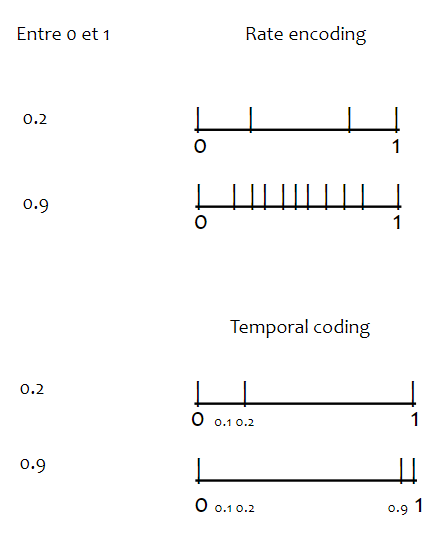
\includegraphics[width=10cm]{./images/ratetempcod.png}
\caption{Encodage des entrées : En haut : le codage temporel, En bas : le codage en fréquence, }
\end{figure}

\hypertarget{couche-de-sortie}{%
\paragraph{Couche de sortie}\label{couche-de-sortie}}

Encore une fois, la couche de sortie fonctionne sur le principe comme
présenté précédemment, avec quelques spécificités : Disons qu'un exemple
a été présenté au réseau dans une fenêtre temporelle \([0,T]\). Il faut
laisser aux impulsions le temps de se propager jusqu'à la couche de
sortie. On va donc observer chaque neurone de sortie sur une fenêtre
\([0, T_2]\), avec \(T_2 > T\).

On pourra alors prendre une décision selon deux stratégies (on parle de
stratégie de \textbf{readout}): - Le neurone retenu est celui qui a
spiké le plus souvent - Le neurone retenu est celui qui a spiké le
premier

\hypertarget{principe-dapprentissage-des-poids-et-architectures}{%
\paragraph{Principe d''apprentissage des poids et
architectures}\label{principe-dapprentissage-des-poids-et-architectures}}

On retrouve les mêmes variétés d'architectures pour les réseaux
impulsionnels que pour les réseaux classiques. En ce qui concerne
l'apprentissage des poids, les techniques sont bien moins maitrisées que
dans le cas des réseaux classiques. En particulier, il n'existe pas de
consensus sur un choix conjoint efficace de l'architecture, du codage
d'entrée, du codage de sortie et de la méthode
d'apprentissage\footnote{C'est ce qui en fait un domaine de recherche très exaltant}.

Ces points dépassent de loin le cadre de ce stage mais sont le coeur de
l'activité du groupe \textbf{Spikes}.

Voyons maintenant le simulateur que j'ai eu à utiliser. \#\# Simulateur
de neurone

Pour pouvoir appliquer et optimiser tous les principes décrit plus haut,
l'utilisation d'un \textbf{simulateur de neurones} est incontournable.
Le simulateur que j'avais à tester s'appelle \textbf{N2S3} (surnommé
\emph{Nessie}).

Néanmoins, avant de parler du simulateur et des tests effectués, je vais
présenter brièvement le language dans lequel \textbf{N2S3} est programmé
: le langage Scala.

\hypertarget{language-de-programmation-scala}{%
\subsection{Language de programmation
Scala}\label{language-de-programmation-scala}}

Scala est un langage de programmation développé par l'équipe de Martin
Odersky à l'École polytechnique fédérale de Lausanne en Suisse depuis
2003.

\begin{figure}[h!]
\label{fig:scala-logo}
\centering
\includegraphics[width=5cm]{./images/scala-logo.png}
\caption{Logo de Scala}
\end{figure}

L'objectif affiché de Scala est d'être une version plus moderne de Java.
En particulier, le gros succès de Java est lié au déploiement de sa
machine virtuelle (la \textbf{jvm}) sur tous les environnements qui rend
les programmes Java extrêmement portables. De fait, Scala est compilé
pour s'exécuter sur la \textbf{jvm}.

L'autre avantage de Java est sa bibliothèque de classe très fournie.
Scala s'exécutant sur la jvm, il est en principe très facile d'utiliser
les objets Java en Scala (dans la pratique, nous ne l'avons pas fait).

Pour concurrencer Java, Scala permet surtout de produire du code
beaucoup plus concis. Il s'appuie également sur trois paradigmes de
programmation :

\begin{itemize}
\tightlist
\item
  La programmation orientée objet, qui reprend la plupart des concepts
  de fonctionnement du langage Java.
\item
  La programmation impérative.
\item
  La programmation fonctionnelle. (Bien qu'elle s'oppose en tout point à
  la programmation impérative, Scala propose de travailler soit avec
  l'une, soit avec l'autre, soit avec les deux).
\end{itemize}

En résumé, Scala est bien un langage objet-fonctionnel-impératif :

\begin{itemize}
\tightlist
\item
  L'architecture des programmes écrits en Scala repose sur des classes.
\item
  Scala fournit tout une suite d'outils pour faire de la programmation
  fonctionnelle.
\item
  Scala autorise tout de même la programmation impérative pour ne pas
  dérouter les nouveaux venus : variables mutables et boucle while.
\end{itemize}

Le langage Scala commence à être utilisé dans l'industrie : plusieurs
entreprises ont annoncées le passage de certaines de leurs applications
au langage Scala, comme Twitter ou le journal The Guardian. Un framework
web nommé «Lift» basé sur Scala a lui aussi vu le jour.

Scala pourrait donc dans le futur s'imposer comme un language de
programmation pratique pour ses possibilités multiples mais aussi sa
portabilité des programmes utilisables sur la machine virtuelle Java.

Bien évidemment, Scala possède un compilateur, un outil de gestion de
projets \textbf{sbt} et peut s'intégrer dans des IDE tels
qu'\textbf{Eclipse} ou \textbf{IntelliJ}.

Présentons maintenant le simulateur \textbf{N2S3}

\hypertarget{n2s3-nessie}{%
\subsection{N2S3 (Nessie)}\label{n2s3-nessie}}

\begin{figure}[h!]
\label{fig:logo-n2s3}
\centering
\includegraphics[width=5cm]{./images/logo-n2s3.png}
\caption{Logo de N2S3}
\end{figure}

\hypertarget{pruxe9sentation-de-n2s3}{%
\subsection{Présentation de N2S3}\label{pruxe9sentation-de-n2s3}}

N2S3 est un simulateur de réseaux de neurones impulsionnels développé
par l'IRCICA de l'université de Lille, téléchargeable, et contenant plus
d'info en détaillé ici \url{https://sourcesup.renater.fr/wiki/n2s3}
dédié à l'apprentissage automatique. Il intègre donc du code
correspondant à deux grandes fonctions.

Tout d'abord, \textbf{N2S3} intègre un moteur du réseau de neurones :
Cette partie permet de créer des neurones et les connecter. Le
simulateur se charge de propager alors automatiquement les spikes à
travers l'architecture. L'autre simulateur testé pendant mon stage par
le stagiaire de M2 (\textbf{NEST}) intègre bien évidemment ces
fonctionnalités.

De plus, \textbf{N2S3} implémente également des simulations
d'apprentissages : Plusieurs méthodes d'encodage des entrées sont déjà
écrites. De plus, le calage temporel de la présentation des différents
exemples de la base existe également. Enfin, on dispose d'exemples
utilisant quelques méthodes d'apprentissage des poids. C'est cette
portion de \textbf{N2S3}, absente de \textbf{NEST} qui fait l'un de ses
points forts.

Durant ce stage, mon objectif était d'installer \textbf{N2S3}, de tester
son utilisation et d'aider le groupe \textbf{Spikes} à comparer ce
simulateur à l'autre possibilité qu'ils envisageait.

La partie installation et utilisation a fait l'objet de la rédaction
d'un tutoriel dans l'annexe \ref{le-tutoriel-n2s3} fourni en pièce
jointe de ce rapport. Dans ce rapport, je vais me concentrer sur la
partie comparaison avec \textbf{NEST} qui a nécessité des choix.

\hypertarget{comparaison-avec-nest}{%
\subsection{Comparaison avec NEST}\label{comparaison-avec-nest}}

\begin{figure}[h!]
\label{fig:nest-logo}
\centering
\includegraphics[width=5cm]{./images/nest-logo.png}
\caption{Logo de NEST}
\end{figure}

\textbf{N2S3}, lorsqu'on le télécharge, et fourni avec de nombreux
exemples. Passée l'installation et la joie de voir ces exemples
fonctionner, il s'agissait d'utiliser ces exemples afin de pouvoir
comparer les performances de \textbf{N2S3} et celles de \textbf{NEST}.

Comme dit plus haut, \textbf{NEST} n'intègre pas de code permettant
facilement de simuler des situations d'apprentissage automatique. Pour
pouvoir comparer ces deux simulateurs, il fallait donc trouver un
exemple que l'on puisse facilement implémenter avec NEST. La suggestion
du groupe \textbf{Spikes} à été d'utiliser un exemple de code
d'apprentissage \textbf{non nonsupervisé} appliqué à la base MNIST
(celle ci est décrite en annexe \ref{la-base-mnist}).

Nous avons donc repris l'exemple \textbf{exempleMNIST} fournit avec
\textbf{N2S3} auquel nous avons ajouté un timer pour pouvoir comparer
les performances des deux simulateurs en termes de temps de calcul.
L'autre stagiaire s'est chargé d'implémenter cette simulation sur NEST.

\hypertarget{description-de-la-simulation-utilisuxe9e-pour-les-tests.}{%
\subsubsection{Description de la simulation utilisée pour les
tests.}\label{description-de-la-simulation-utilisuxe9e-pour-les-tests.}}

La simulation se base donc sur la base \textbf{MNIST}, se composant
d'images de 28x28 pixels, vues comme 784 caractéristiques. Cette base
sert pour les test de reconnaissance manuscrite, elle possède 60 000
images pour l'apprentissage et 10 000 pour les tests.

L'architecture de la simulation est la suivante : - 784 neurones
d'entrée - une trentaine de neurones de sortie - la couche d'entrée est
connectées directement et de façon complète à la couche de sortie.

Ces neurones de sortie doivent apprendre, de façon non supervisée, à se
spécialiser sur certains chiffres. Pour cela :

La connection entre la couche d'entrée et la couche de sortie est faite
par des synapses qui mettant en oeuvre un mécanisme dit
\textbf{simplified STDP}. Ce mécanisme est responsable de
l'apprentissage non supervisé et décrit brièvement en annexe
(\ref{apprentissage-supervisuxe9}). Ce mécanisme modifie les poids d'un
neurone pour renforcer les connections utiles et affaiblir les
connections inutiles. En effet, pour décrire un chiffre en particulier,
seuls quelques pixels sont importants.

Il faut également empêcher les neurones de se spécialiser sur les mêmes
chiffres. Pour cela, le mécanisme du \textbf{Winner-take-all} est
utilisé : Quand un neurone de sortie \textbf{spike}, il inhibe les
autres neurones de la couche de sortie. Ceux ci étant inhibés, il
n'apprendront rien de cet exemple et pourront apprendre sur d'autres.
Pour mettre en oeuvre ce mécanisme, les 30 neurones qui composent la
couche de sortie sont interconnectés entre eux par des connections
inhibitrices (de poids négatifs). Ce mécanisme est décrit dans l'annexe
(\ref{apprentissage-supervisuxe9})

Le principe de la simulation est que les images sont converties en
impulsions et injectées par les neurones d'entrée, puis à chaque neurone
de sortie au fur et à mesure que les 60 000 images d'apprentissage sont
injectées, une spécialisation s'effectue. Chacun des neurones se
spécialise sur la détection d'un chiffre de 0 à 9.

Il nous a semblé important que le lecteur puisse évaluer la complexité
du code d'une telle simulation. Voici donc un bref exemple de code du
simulateur (en Scala).

\begin{figure}[h!]
\label{fig:code}
\centering
\includegraphics[height=5cm]{./images/code01.jpg}
\caption{Bout de code}
\end{figure}

Je vais essayer de décrire ce que fait cette portion de code :

\begin{itemize}
\tightlist
\item
  Déclarations de notre réseau de neurone
\item
  Création de flux d'entrée de Stream (Choix de codage de chaque pixel,
  une intensité, la fréquence pour les nombres de spikes)
\item
  Création de la couche d'entrée par rapport au image et label qu'on va
  injecter dans le canal pour les test des neurones
\item
  Création de notre couche de sortie
\item
  Connection entre couche d'entrée et de sorte
\item
  Création du réseau de neurones
\end{itemize}

\hypertarget{ruxe9sultats-obtenus}{%
\subsubsection{Résultats obtenus :}\label{ruxe9sultats-obtenus}}

La simulation existait dans les exemples, notre travail de développement
a donc tout d'abord seulement consisté a faire fonctionner le simulateur
et ses exemples. Nous avons ensuite ajouté le chronomètre dans ce code.

Enfin, j'ai exploré une fonctionnalités des projets Scala, non incluse
dans N2S3, qui nous a permis de produire un executable utilisable sur
tout machine disposant d'une jvm. Nous avons pu ainsi faire tourner
notre exemple sur différentes machines :

\begin{itemize}
\tightlist
\item
  un pc linux
\item
  différents pc windows
\item
  le cluster de calcul du c3i.
\end{itemize}

Pour comparer les temps de calculs de NEST et N2S3 sur la même machine,
nous avons fourni cet exécutable au second stagiaire qui a ainsi pu
faire tourner les 2 simulateurs sur sa machine (machine virtuelle
linux).

Nous avons ainsi mesuré le temps nécessaire pour faire tourner
l'ensemble des exemples de la base MNIST.

\begin{table}[h!]
\centering
\begin{tabular}{|c|c|c|c|}
\hline
base & nombre d'exemples & temps N2S3 & temps NEST \\
\hline
train & 60 000 & 1h29mn & 3h13min \\
\hline
test & 10 000 & 18min & 39min \\
\hline
\end{tabular}
\caption{\label{tab:tempsMnist} Temps de calculs}
\end{table}

Voyons maintenant tout ce qui m'a été appris niveau outils et méthode de
travail \#\# Outils et méthodes de travail

De façon générale, le choix des outils est toujours conditionné par le
contexte dans lequel ces outils sont employés. Nous reviendrons sur
cette idée pour justifier chacun des choix que nous avons fait lors de
ce stage. Mais pour commencer, il me faut décrire brièvement ce
contexte, plus particulièrement les conditions du stage.

\hypertarget{le-travail-au-lamia}{%
\subsection{Le travail au LAMIA}\label{le-travail-au-lamia}}

Avant toutes choses, pendant toute la période du stage, mon stage a été
encadré de très près par mon tuteur, ce qui se justifie par la
complexité des problèmes abordés. J'ai ainsi bénéficié de l'aide de mon
tuteur, ou encore de l'aide complémentaire du stagiaire de M2.

Je travaillais dans le bureau de \textbf{Mr.~Vincent PAGÉ} muni de mon
ordinateur portable personnel.\\
Chaque fin de semaine était rythmé par la présentation orale des travaux
effectués durant la semaine, devant les membres du groupe
\textbf{Spikes}.

Ce stage avait donc, au delà d'un objectif de développement, de produire
de la documentation pour le groupe \textbf{Spikes}, documentation à
archiver et modifier sur le long terme.

Je vais donc pouvoir passer aux différents outils qui m'ont été proposés
et avec lesquels j'ai travaillé durant tout mon stage. Chacun de ces
outils avait pour objectif d'accroitre ma productivité et de permettre
cet archivage, sans nécessiter de formation trop longue, le stage ne
durant que quatre semaines.

\hypertarget{outils-de-gestion-de-version-git-gitkraken-gitlab}{%
\subsection{Outils de gestion de version (Git, GitKraken,
GitLab)}\label{outils-de-gestion-de-version-git-gitkraken-gitlab}}

\begin{figure}[h!]
\label{fig:gitkraken}
\centering
\includegraphics[height=5cm]{./images/gitlab-gitkraken.png}
\caption{Logo GitKraken et GitLab}
\end{figure}

Git est le logiciel de gestion de version le plus utilisé au monde. Il
peut être utilisé pour archiver l'évolution d'un logiciel, mais aussi
d'une documentation. C'est donc tout naturellement que nous sommes
tournés vers lui pour conserver une trace de mon passage dans le groupe
\textbf{Spikes}.

Il peut être utilisé en local sur une machine, mais prend tout son
intérêt lorsque l'on dispose d'un serveur permettant de travailler
depuis différentes machines, éventuellement à plusieurs.

Dans ce cas, le principe est de pouvoir garder sur un serveur, toutes
les modifications liées à un répertoire (\textbf{le projet}). Ainsi la
récupération de fichier est plus facile si par malheur vous le
supprimez, ou pour revenir à un moment fonctionnel d'un programme par
exemple.\\
Dans notre cas , le serveur Git est le GitLab du LAMIA
\url{http://lic3i.univ-ag.fr}. Pour les travaux sur \textbf{N2S3}, mon
tuteur a créé sur ce serveur un dépôt (\textbf{N2S3\_Experiences}), sur
lequel toutes les modifications apportées sur mon ordinateur pouvaient
être repercutées. Ce dépôt contient ainsi une trace de tout ce que j'ai
pu effectuer durant ma période de stage.

Git étant d'un usage assez complexe, nous avons choisi d'utiliser le
client \textbf{GitKraken} qui permet d'utiliser git via une interface
graphique et rend l'utilisation beaucoup plus ergonomique pour un stage
court.

Ci dessous, une illustration de l'avancement du projet
\textbf{N2S3\_Experiences}. La découverte de Git s'est faite avec l'aide
de mon tuteur ainsi qu'en consultant principalement le site \cite{git}.

\begin{figure}[h!]
\label{fig:gitkrakenUsage}
\centering
\includegraphics[height=5cm]{./images/gitkraken.png}
\caption{Capture d'écran du projet N2S3 Experiences}
\end{figure}

\hypertarget{markdown-latex}{%
\subsection{Markdown + LATEX}\label{markdown-latex}}

Le lecteur aura peut être noté que ce rapport de stage a été rédigé en
\textbf{LaTeX}. Latex est un langage de description de documents très
utilisé pour la rédaction d'articles et de rapports. Ses intérêts
majeurs par rapport à des traitements de textes tels que World sont : -
le fichier latex est un fichier texte (notamment archivable plus
efficacement avec GIT) - Il produit des documents plus professionnels
car le compilateur LaTeX suit les règles de typographie standards.

En revanche, La rédaction en LaTeX suppose un temps non négligeable
d'apprentissage. De ce fait, mon tuteur m'a proposé de rédiger mon
rapport en \textbf{Markdown} lequel est converti en LaTeX grâce au
logiciel de conversion en ligne de commande \textbf{Pandoc}.

Markown est un langage beaucoup plus simple que LaTeX. Il n'a en
revanche pas la même souplesse, mais il est possible de taper du code
LaTex dans le fichier Markdown pour toutes les opérations un peu
délicates.

Voici un exemple de fichier markdown

\begin{lstlisting}
# Un titre

## Un titre de niveau Deux

- une liste a puces
- composee d elements
\end{lstlisting}

Comme on le voit, cette syntaxe est directement lisible et facilite
grandement la rédaction, surtout si l'on compare avec le code latex
correspondant :

\begin{lstlisting}
\section{Un titre}\label{un-titre}}

\subsection{Un titre de niveau Deux}

\begin{itemize}
\item
  une liste a puces
\item
  composee d elements
\end{itemize}
\end{lstlisting}

La chaine complète est décrite ci dessous :

\begin{enumerate}
\def\labelenumi{\arabic{enumi}.}
\tightlist
\item
  Séparation du document final en page de garde + table des matières
  chapitres (ou sections) + biblio + annexes.\\
\item
  La page de garde a elle été directement écrite en LATEX (suivant un
  exemple pré-existant).
\item
  Puis on rédige chacune des sections en Markdown avec l'éditeur de
  texte \textbf{Atom} qui m'a été conseillé.
\item
  conversion de chaque section Markdown -\textgreater{} LaTeX
\item
  Compilation des différentes portions du rapport (full LaTeX)
  -\textgreater{} pdf grâce a \textbf{pdflatex}.
\end{enumerate}

Tout ceci produit le rapport final que le lecteur a sous les yeux.
L'ensemble de ces étapes est executé par un script \textbf{batch} pour
Windows, ce qui rend l'ensemble de l'opération très simple.

Pour les transparents que je présentais, chaque semaine, nous avons
classiquement utilisé Powerpoint, bien que l'on puisse également
appliquer le même genre de chaine de traitement a partir de Markdown.
Mon tuteur étant moins à l'aise dans la création de transparents depuis
Markdown, à court terme, il nous a semblé préférable de ne pas retenir
cette solution.
